\section{História da linguagem}

No começo da decada de 90 um pequeno grupo de engenheros da Oracle chamados de ''Green Team'' acreditava que a próxima onde de na area da computação seria a união de equipamentos eletroeletrônicos com os computadores. O ''Green Team'' liderado por James Gosling, demonstraram que a linguagem de programaçao Java, que foi desenvolvida pela equipe e originalmente era chamado de Oak, foi desenvolvida para dispositivos de entretenimento como aparelhos de tv a cabo, porem não foi bem aceita no meio. Em 1995 com a massificação da Internet, a linguagem Java teve sua primeira grande aplicação o navegador Netscape.

Java é uma linguagem de programação de propósito geral orientada a objetos, concebida especificadademente para ter poucas dependencias de implementação que isso acarreta que uma vez que a aplicação fora desenvolvida ela poderá ser executada em qualquer ambiente computacional.

Na sua primeira versão chamada de Java 1 (\acs{JDK} 1.0.2) haviam oito pacotes básicos do java como: java.lang, java.io, java.util, java.net, java.awt, java.awt.image, java.awt.peer e java.applet. Foi usado para o desenvolvimento de ferramentas populares na epoca como o Netscape 3.0 e o Internet Explorer 3.0.

Sua segunda versão foi o \acs{JDK}1.1 \cite{JDK1.1} que trouxe ganhos em funcionalidades, desempenho e qualidade. Novas aplicações tambem surgiram como : JavaBeans, aprimoramento do \acs{AWT}, novas funcionalidades como o \acs{JDBC}, acesso remoto ao objeto \acs{RMI} e suporte ao padrão Unicode 2.0.

A terceira versão Java 2 (\acs{JDK} 1.2) ofereceu melhorias significativas no desempenho, um novo modelo de segurança, flexível e um conjunto completo de aplicações de programação interfaces \acs{API}'s. Os novos recursos da plataforma Java 2 incluiram: 
\begin{itemize}
  \item O modelo de "sandbox"  foi ampliado para dar aos desenvolvedores, usuários e administradores de sistema a opção de especificar e gerenciar um conjunto de políticas de segurança flexíveis que governam as ações de uma aplicação ou applet que pode ou não ser executada.
  \item Suporte nativo a thread para o ambiente operacional Solaris. Compressão de memória para classes carregadas. Alocação de memória com mais desempenho e melhor para a coleta de lixo. Arquitetura de máquina virtual conectável para outras máquinas virtuais, incluindo a Java HotSpot VMNew. Just in Time (JIT). Java Native Interface \acs{JNI} de conversão.
  \item O conjunto de componentes de projeto, \acs{GUI} (Swing). \acs{API} Java 2D que fornece novos recursos gráficos 2D e \acs{AWT}, bem como suporte para impressão. O Java {\it look and fell}. Uma nova API de acessibilidade.
  \item Framework de entrada de caracteres (suporte a japonês, chinês e coreano). Complexo de saída usando a \acs{API} do Java 2D para fornecer um {\it display} bi-direcional, de alta qualidade de japonês, árabe, hebraico e outras línguas de caracteres.
  \item Java Plug-in para navegadores da web, incluída na plataforma Java 2, fornecendo um tempo de execução totalmente compatível com a máquina virtual Java amplamente implantadas em navegadores.
  \item Invocação das operações ou serviços de rede remoto. Totalmente compatível com Java ORB e incluído no tempo de execução.
  \item \acs{JDBC} que fornece um acesso mais fácil aos dados para consultas mais flexíveis. Melhor desempenho e estabilidade são promovidos por cursores de rolagem e suporte para SQL3 de tipos.
\end{itemize}

Em 8 de Maio de 2000 foi anunciado o Java 2 versão 1.3 que trouxe ganho de desempenho em relação a primeira versão da JS2E de cerca de 40\%  no tempo de {\it  start-up}. Tambem trouxe novas funcionaliadades como: 

\begin{itemize}
  \item O Java HotSpot VM de cliente e suas bibliotecas atentando ao desempenho ao fazer o J2SE versão 1.3 a {\it realease} o mais rápido até à data.
  \item Novos recursos, como o {\it caching applet} e instalação do pacote opcional Java através da tecnologia Java {\it  Plug-in} para aumentar a velocidade e a flexibilidade com que os {\it applets} e aplicativos baseados na tecnologia Java pode ser implantado. Java {\it  Plug-in} tecnologia é um componente do ambiente de execução Java 2 que permite Java {\it applets} e aplicativos para a execução.
  \item O novo suporte para \acs{RSA} assinatura eletrônica, gerenciamento de confiança dinâmico, certificados X.509, e verificação de arquivos o que significa o aumento das possibilidades que os desenvolvedores tem para proteger dados eletrônicos.
  \item Uma série de novos recursos e ferramentas de desenvolvimento da tecnologia J2SE versão 1.3 que permite o desenvolvimento mais fácil e rápido de aplicações baseadas na tecnologia {\it web} ou Java {\it  standalone} de alto desempenho.
  \item A adição de RMI/IIOP e o JNDI para a versão 1.3, melhora na interoperabilidade J2SE. RMI/IIOP melhora a conectividade com sistemas de {\it  back-end} que suportam CORBA. JNDI fornece acesso aos diretórios que suportam o populares LDAP Lightweight Directory Access Protocol, entre outros.
\end{itemize}

No ano de 2002 no dia 6 de Fevereiro, foi lançado a J2SE versão 1.4. Com a versão 1.4, as empresas puderam usar a tecnologia Java para desenvolver aplicativos de negócios mais exigentes e com menos esforço e em menos tempo. As novas funcionalidades como a nova I/O e suporte a 64 bits. A J2SE se tornou plataforma ideal para a mineração em grande escala de dados, inteligência de negócios, engenharia e científicos. A versão 1.4 forneceu suporte aprimorado para tecnologias padrões da indústria, tais como SSL, LDAP e CORBA a fim de garantir a operacionalidade em plataformas heterogêneas, sistemas e ambientes. Com o apoio embutido para XML, a autenticação avançada, e um conjunto completo de serviços de segurança, está versão forneceu base para padrões de aplicações Web e serviços interoperáveis. O J2SE avançou o desenvolvimento de aplicativos de cliente com novos controles de GUI, acelerou Java 2D, a performance gráfica, internacionalização e localização expandida de apoio, novas opções de implantação e suporte expandido para o até então Windows XP.\\

Com a chegada da \acs{JSE2} versão 1.5 (Java 5.0) em 30 de Setembro de 2004, impulsionou benefícios extensivos para desenvolvedores, incluindo a facilidade de uso, desempenho global e escalabilidade, monitoramento do sistema e gestão e desenvolvimento. O Java 5 foi derivado do trabalho de 15 componentes Java Specification Requests (JSRs) englobando recursos avançados para a linguagem e plataforma. Os líderes da indústria na época que participam no grupo de peritos J2SE 5.0 incluiram: Apache Software Foundation, Apple Computer, BEA Systems, Borland Software Corporation, Cisco Systems, Fujitsu Limited, HP, IBM, Macromedia, Nokia Corporation, Oracle, SAP AG, SAS Institute, SavaJe Technologies e Sun Microsystems.

Novas funcionalidades foram implementadas como:

\begin{itemize}
  \item Facilidade de desenvolvimento: os programadores da linguagem Java pode ser mais eficiente e produtivos com os recursos de linguagem Java 5 que permitiram a codificação mais segura. Nesta versão surgiu o {\it Generics} ~\cite{OracleGenerics, bracha1998gj}, tipos enumerados, metadados e autoboxing de tipos primitivos permitindo assim uma fácil e rápida codificação.
  
  \item Monitoramento e gestão: Um foco chave para a nova versão da plataforma, a aplicativos baseados na tecnologia Java {\it Virtual Machine} que passou a ser monitorado e gerenciado com o {\it built-in} de suporte para Java {\it Management Extensions}. Isso ajudou a garantir que seus funcionários, sistemas de parceiros do cliente permanecessem em funcionamento por mais tempo. Suporte para sistemas de gestão empresarial baseados em SNMP também é viável.
  
  \item Um olhar novo aplicativo, mais moderna, baseada na tecnologia Java padrão e proporciona uma sensação GUI para aplicativos baseados na tecnologia Java. A J2SE 5.0 teve suporte completo a internacionalização e também possuindo suporte para aceleração de hardware por meio da API OpenGL e tambem para o sistema operacional Solaris e sistemas operacionais da distribuição Linux.
  
  \item Maior desempenho e escalabilidade: A nova versão incluiu melhorias de desempenho, tais como menor tempo de inicialização, um menor consumo de memória e JVM auto ajustável para gerar maior desempenho geral do aplicativo e desenvolvimento em J2SE 5.0 em relação às versões anteriores.
\end{itemize}

Java 1.6 (Java 6) foi divulgado em 11 de dezembro de 2006. Tornou o desenvolvimento mais fácil, mais rápido e mais eficiente em termos de custos e ofereceu funcionalidades para serviços web, suporte linguagem dinâmica, diagnósticos e aplicações desktop. Com a chegada dessa nova versão do Java houve combinação com o NetBeans IDE 5.5 fornecendo aos desenvolvedores uma estrutura confiável, de codigo aberto e compatível, de alta performance para entregar aplicativos baseados na tecnologia Java mais rápido e mais fácil do que nunca. O NetBeans IDE fornece uma fonte aberta e de alto desempenho, modular, extensível, multi-plataforma Java IDE para acelerar o desenvolvimento de aplicações baseadas em software e serviços {\it web}.
Novas funcionalidades foram implementadas como:

\begin{itemize}
  \item O Java 1.6 ajudou a acelerar a inovação para o desenvolvedor, aplicativos de colaboração {\it online} e baseadas na {\it web}, incluindo um novo quadro de desenvolvedores \acs{API}'s para permitir a mistura da tecnologia Java com linguagens de tipagem dinâmica, tais como PHP, Python, Ruby e tecnologia JavaScript. A Sun também criou uma coleção de mecanismos de script e pré-configurado o motor JavaScript Rhino na plataforma Java. Além disso, o software inclui uma pilha completa de clientes de serviços web e suporta as mais recentes especificações de serviços {\it web}, como \acs{JAX-WS} 2.0, \acs{JAXB} 2.0, \acs{STAX} e \acs{JAXP}.
  \item A plataforma Java 1.6 forneceu ferramentas expandidas para o diagnóstico, gestão e monitoramento de aplicações e também inclui suporte para o novo NetBeans Profiler 5.5 para Solaris DTrace e, uma estrutura de rastreamento dinâmico abrangente que está incluído no sistema operacional Solaris 10. Além disso, o software Java SE 6 aumenta ainda mais a facilidade de desenvolvimento com atualizações de interface ferramenta para o Java Virtual Machine (\acs{JVM}) e o Java Platform Debugger Architecture (\acs{ACDP}).
\end{itemize}

Java 7 ~\cite{JSE7} foi lançado no dia 28 de julho de 2011. Essa versão foi resultado do desenvolvimento de toda a indústria envolvendo uma revisão de codigo aberto e extensa colaboração entre os engenheiros da {\it Oracle} e membros do ecossistema Java em todo o mundo através da comunidade {\it OpenJDK} e do {\it Java Community Process} (\acs{JCP}). Compatibilidade com versões anteriores de Java 7 com versões anteriores da plataforma a fim de preservar os conjuntos de habilidades dos desenvolvedores de software Java e proteger os investimentos em tecnologia Java.

Com essa versão novas funcionalidades foram adicionadas:

\begin{itemize}
  \item As alterações de linguagem ajudaram a aumentar a produtividade do desenvolvedor e simplificar tarefas comuns de programação, reduzindo a quantidade de código necessário, esclarecendo sintaxe e tornar o código com mais legibilidade.
  \item Melhor suporte para linguagens dinâmicas incluindo: Ruby, Python e JavaScript, resultando em aumentos substanciais de desempenho no \acs{JVM}.
  \item Uma nova API {\it multicore-ready} que permite aos desenvolvedores para se decompor mais facilmente problemas em tarefas que podem ser executadas em paralelo em números arbitrários de núcleos de processador.
  \item Uma interface de I/O abrangente para trabalhar com sistemas de arquivos que podem acessar uma ampla gama de atributos de arquivos e oferecem mais informações quando ocorrem erros.
  \item Novos recursos de rede e de segurança. Suporte expandido para a internacionalização, incluindo suporte a Unicode 6.0. Versões atualizadas das bibliotecas padrão.\\
\end{itemize}

Com o lançamento do Java SE 8 em 18 de Março de 2014, permitiu uma maior produtividade e desenvolvimento de aplicativos significativos aumentos de desempenho através da redução de linhas de código, {\it collectons} melhoradas, modelos mais simples de programação paralela e uso mais eficiente de processadores multi-core modernos.As principais características do \acs{JDK} 8 são o Projeto Lambda, Nashorn JavaScript Engine, um conjunto de perfis compactas e a remoção da "geração permanente" do HotSpot Java Virtual Machine (\acs{JVM}). A \acs{JDK} 8 alcançou desempenho recorde mundial para 4 sistemas de soquete em servidores baseados em Intel e NEC por 2 sistemas de soquete em servidores SPARC da Oracle T5, com uma melhoria de desempenho de 12\% para 41\% em comparação com o JDK 7 na mesma configuração de Oracle.
O \acs{JDK} 8 adicionou novas funcionalidades como:
  \begin{itemize}
  \item As expressões lambda são suportados pelas seguintes características: As referências a metodos são compactas, maior legibilidade expressões lambda para métodos que já têm um nome. Métodos padrão que permitem adicionar novas funcionalidades para as interfaces de suas bibliotecas e assegurar a compatibilidade binária com o código escrito para versões mais antigas dessas interfaces. Eles são os métodos de interface que têm uma aplicação e a palavra-chave padrão no início da assinatura do método. Além disso, pode-se definir métodos estáticos em interfaces. Novos e aprimorados APIs que se aproveitam de expressões lambda e dos {\it streams} em Java 8 descrevem as classes novos e aprimorados que se aproveitam de expressões lambda e {\it streams}.
  \item O compilador Java aproveita digitação alvo para inferir os parâmetros de tipo de um método de invocação genérica. O tipo de destino de uma expressão é o tipo de dados que o compilador Java espera, dependendo de onde a expressão aparece. Por exemplo, você pode usar o tipo de destino de uma instrução de atribuição para o tipo de inferência em Java 7. No entanto, em Java 8, você pode usar o tipo de destino para a inferência de tipos em mais contextos.
  \item Anotações sobre tipos Java. Agora é possível aplicar uma anotação em qualquer lugar onde um tipo é usado. Utilizado em um conjunto com um sistema de tipo de conector, isso permite a verificação de tipo mais forte de seu código.
  \item  Repetindo Anotações. Agora é possível aplicar o mesmo tipo de anotação mais de uma vez para a mesma declaração ou o tipo de utilização.
  \end{itemize}


								
%\chapter{Fundamentação}
\section {Aspectos evolutivos da liguagem Java}
		\subsection {Java 2}
			A primeira versão do Java Security, disponível no \acs{JDK} 1.1 \cite{JDK1.1}, contém um subconjunto dessa funcionalidade, incluindo \acs{API}'s para:
		  \begin{itemize}
			  \item Assinaturas Digitais: Algoritmos de assinatura digital, como \acs{DSA} ou \acs{MD5} com \acs{RSA}. A funcionalidade inclui a geração de chaves público/privado , bem como assinatura e verificação de dados digitais.
			  \item Gerenciamento de Chaves: Um conjunto de abstrações para o gerenciamento de ''diretores'' (entidades como usuários individuais ou grupos), suas chaves, e os seus certificados. Ele permite que aplicativos para projetar seu próprio sistema de gerenciamento de chaves, e para interoperar com outros sistemas em alto nível.
			  \item Lista de controle de acesso: Um conjunto de abstrações para o gerenciamento de ''diretores'' e suas permissões de acesso.
			  \item A obtenção de um objeto de assinatura: 
			  
\begin{lstlisting}
import java.security.Signature;
import java.security.NoSuchAlgorithmException;
	
public class SignFile {
	Signature signature;
		
	private void init(String algorithm) throws NoSuchAlgorithmException{
		signature = Signature.getSignature(algorithm);
    }
}
\end{lstlisting}
			  
			  \item Em versões anteriores, Java suportava apenas {\it top-level} classes, que devem ser membros de pacotes. Na versão 1.1, o programador Java pode agora definir classes internas como membros de outras classes ~\cite{bracha1998gj}, localmente dentro de um bloco de instruções, ou (anonimamente) dentro de uma expressão.
		  
\begin{lstlisting}
public class FixedStack {
	...
	 public java.util.Enumeration elements() {
	     return new FixedStack$Enumerator(this);
	 }
}
		
class FixedStack$Enumerator implements java.util.Enumeration {
	private FixedStack this$0;
	
	FixedStack$Enumerator(FixedStack this$0) {
		this.this$0 = this$0;
		this.count = this$0.top;
	 }
			
	int count;
	public boolean hasMoreElements() {
		return count > 0;
	}
		
	public Object nextElement() {
		if (count == 0)
			throw new NoSuchElementException("FixedStack");
		
		return this$0.array[--count];
	}
}
\end{lstlisting}
			
			\clearpage
			\item Para escrever um objeto remoto \acs{RMI}, escreve-se uma classe que implementa uma ou mais interfaces remotas. 
			
\begin{lstlisting}
package examples.hello;
public interface Hello extends java.rmi.Remote {
	String sayHello() throws java.rmi.RemoteException;
}
\end{lstlisting}
	 
\item HelloImpl.java
\begin{lstlisting}
package examples.hello;

import java.rmi.;
import java.rmi.server.UnicastRemoteObject;

public class HelloImpl extends UnicastRemoteObject implements Hello{
	private String name;
	
	public HelloImpl(String s) throws RemoteException {
		super();
		name = s;
	}
	
	public String sayHello() throws RemoteException {
		return  "Hello World!";
	}
	
	public static void main(String args[]){
	
		System.setSecurityManager(new RMISecurityManager());
	
		try {
			HelloImpl obj = new HelloImpl("HelloServer");
			Naming.rebind("//myhost/HelloServer", obj);
			System.out.println("HelloServer bound in registry");
		} catch (Exception e) {
			System.out.println("HelloImpl err: " + e.getMessage());
			e.printStackTrace();
		}
	}
}
\end{lstlisting}
		\end{itemize}


	\clearpage
	\subsection {Java 4}
	  \begin{itemize}
		  \item {\it Assertion Facility} \cite{JSE8_Enhancements}. As {\it assertions} são expressões booleanas que o programador acredita ser verdade sobre o estado de um programa de computador. Por exemplo, depois de ordenar uma lista o programador pode afirmar que a lista está em ordem crescente. Avaliando as afirmações em tempo de execução para confirmar a sua validade é uma das ferramentas mais poderosas para melhorar a qualidade do código, uma vez que rapidamente se descobre equívocos do programador sobre o comportamento de um programa.
	  \end{itemize}
	
	\subsection {Java 5}
	  \begin{itemize}
		  \item {\it Generics} \cite{JSE8_Enhancements, OracleGenerics, Parnin:ACM2011}. Este novo recurso para o sistema de tipo permite que um tipo ou método operar em objetos de vários tipos, proporcionando em tempo de compilação tipo de segurança. Acrescenta em tempo de compilação um tipo de segurança para as {\it collections} e elimina o trabalho penoso de {\it casting}. Um exemplo do uso de {\it collections} e {\it generics} respectivamente:
\begin{lstlisting}
static void expurgate(Collection c) {
	for (Iterator i = c.iterator(); i.hasNext(); )
		if (((String) i.next()).length() == 4)
			i.remove();
	}
	
static void expurgate(Collection<String> c) {
	for (Iterator<String> i = c.iterator(); i.hasNext(); )
		if (i.next().length() == 4)
			i.remove();
}
\end{lstlisting}
		  
		\item {\it For-Each Loop}. Esta nova estrutura de linguagem elimina o trabalho e erro de propensão de iteradores e variáveis de índice quando a iteração ocorre sobre coleções e arrays. Como a construção evoluiu com o advento dessa nova estrutura:
	
\begin{lstlisting}
void cancelAll(Collection<TimerTask> c) {
	for (Iterator<TimerTask> i = c.iterator(); i.hasNext(); )
	   i.next().cancel();
}
	
void cancelAll(Collection<TimerTask> c) {
	for (TimerTask t : c)
		t.cancel();
}
\end{lstlisting}
	  
	  \clearpage
	  \item {\it Varargs}. Esta nova estrutura tende a eliminar a necessidade de passagem manual de listas de argumentos em um array ao invocar métodos que aceitam de um comprimento variável de uma lista de argumentos. Nas versões anteriores, um método levava um número arbitrário de valores necessários a  criar uma matriz e colocar os valores para a matriz antes de chamar o método.


\begin{lstlisting}
public class Test {
	public static void main(String[] args) {
	  int passed = 0;
	  int failed = 0;
	  for (String className : args) {
	      try {
	          Class c = Class.forName(className);
	          c.getMethod("test").invoke(c.newInstance());
	          passed++;
	      } catch (Exception ex) {
	          System.out.printf("%s failed: %s%n", className, ex);
	          failed++;
	      }
	  }
	  System.out.printf("passed=%d; failed=%d%n", passed, failed);
	}
}
\end{lstlisting}
 
	  \item {\it Autoboxing/Unboxing}. Esta nova estrutura elimina o trabalho de conversão manual entre tipos primitivos (como {\it int}) e os tipos de classes {\it wrapper}
  \end{itemize}
  
  
  
	\subsection {Java 6}
		Não ocorram mudanças ou introdução de novas estruturas na linguagem Java ~\cite{JSE8_Enhancements}.
	
	\subsection {Java 7}
		\begin{itemize}
		  \item {\it Multi Catch} e lançamento de exceções com melhora na verificação de tipos. Um único bloco {\it catch} poderá lidar com mais de um tipo de exceção. Além disso, o compilador executa a análise mais precisa das exceções. Isso permite que o programador especifique tipos de exceção mais específicos na cláusula de uma declaração método. Um exemplo de como era as estruturas que usavam {\it cacths} e com a introdução de {\it multi catch} com o Java 7 ~\cite{JSE7}, respectivamente.
  

\begin{lstlisting}
catch (IOException ex) {
	logger.log(ex);
	throw ex;
}catch (SQLException ex) {
	logger.log(ex);
	throw ex;
}
\end{lstlisting}
\clearpage
\begin{lstlisting}
catch (IOException|SQLException ex) {
	logger.log(ex);
	throw ex;
}
\end{lstlisting}


 \item O {\it try-with-resouces}. A declaração {\it try-with-resouces} é uma instrução {\it try} que declara um ou mais recursos. Um recurso é um objeto que deve ser fechada após o programa terminar com ele. Essa declaração garante que cada recurso é fechada no final da declaração ~\cite{JSE7_Advanced}.
	 
\begin{lstlisting}

public static void writeToFileZipFileContents(
			String zipFileName, String outputFileName) throws java.io.IOException {
	
	java.nio.charset.Charset charset = java.nio.charset.StandardCharsets.US_ASCII;
	java.nio.file.Path outputFilePath = java.nio.file.Paths.get(outputFileName);
	
	try(
		 java.util.zip.ZipFile zf = new java.util.zip.ZipFile(zipFileName);
		 java.io.BufferedWriter writer = java.nio.file.Files.newBufferedWriter(outputFilePath, charset)
	){
	
		for (java.util.Enumeration entries = zf.entries(); entries.hasMoreElements();) {
			 String newLine = System.getProperty("line.separator");
			 String zipEntryName = ((java.util.zip.ZipEntry)entries.nextElement()).getName() + newLine;
			 writer.write(zipEntryName, 0, zipEntryName.length());
		 }
	}
}

\end{lstlisting}
		  
		  \clearpage
		  \item Inferência de tipos para criação de instâncias em {\it generics} \cite{OracleGenerics,bracha1998gj,Parnin:ACM2011}. Com o Java 7 pode-se substituir os argumentos de tipo necessários para invocar o construtor de uma classe genérica com um conjunto vazio de parâmetros de tipo (<>), desde que o compilador infira os argumentos de tipo a partir do contexto. Este par de colchetes angulares é informalmente chamado de diamante.
  
  

\begin{lstlisting}
Map<String, List<String>> myMap = new HashMap<String, List<String>>();
Map<String, List<String>> myMap = new HashMap<>();
	
List<String> list = new ArrayList<>();
list.add("A");

list.addAll(new ArrayList<>());
	
class MyClass<X> {
	<T> MyClass(T t) {
	...
	}
}
\end{lstlisting}
	 
	  \end{itemize}
	  
	  
	\subsection{Java 8}
	  \begin{itemize}
		  \item Melhoria na inferência de tipos. O compilador Java aproveita digitação para inferir os parâmetros de tipo de uma invocação de método genérica. O tipo de destino de uma expressão é o tipo de dados que o compilador Java espera, dependendo de onde a expressão aparece. Por exemplo, pode-se usar o tipo de destino de uma instrução de atribuição para o tipo de inferência em Java 7. No entanto, em Java 8, pode-se usar o tipo de destino para a inferência de tipos em mais contextos. O exemplo mais proeminente está usando tipos de destino de um método de invocação para inferir os tipos de dados dos seus argumentos.

\begin{lstlisting}
	List<String> stringList = new ArrayList<>();
	stringList.add("A");
	stringList.addAll(Arrays.asList());
\end{lstlisting}
		  
		  
		  \item Expressões lambda. Permitem encapsular uma única unidade de comportamento e passá-lo para outro código. Pode-se usar uma expressãos lambda, se quiser uma determinada ação executada em cada elemento de uma {\it collection}, quando o processo for concluído, ou quando um processo encontra um erro. \cite{JSE7} \\
	  \end{itemize}

\clearpage
\begin{lstlisting}
public class Calculator {
	
	interface IntegerMath {
		int operation(int a, int b);   
	}

	public int operateBinary(int a, int b, IntegerMath op) {
		return op.operation(a, b);
	}

	public static void main(String... args) {

		Calculator myApp = new Calculator();
		IntegerMath addition = (a, b) -> a + b;
		IntegerMath subtraction = (a, b) -> a - b;
		System.out.println("40 + 2 = " + myApp.operateBinary(40, 2, addition));
		System.out.println("20 - 10 = " + myApp.operateBinary(20, 10, subtraction));    
		
	}
}
\end{lstlisting}
\chapter{Fundamentação}
Um ponto crítico quanto a análise de código fonte é o \textit{parser} da linguagem, onde é necessário reconhecer uma frase para efetuar a interpretação ou fazer a tradução. Inicialmente é necessário identificar se a frase que será tratada é um \textit{assignment} ou uma chamada de função.
 
Reconhecer uma frase acarreta em duas coisas, distingui-la de outras construções e identificar os elementos e as subestruturas que compõem esta frase. Por exemplo se uma frase for reconhecida como um \textit{assignment}, pode-se identificar as variáveis a esquerda do operador \textbf{=} e uma expressão que é a subestrutura a direita. Este ato de reconhecer uma frase é denominado \textit{Parse}.

\section{Parse}

Para conceber uma ferramenta de análise de código é necessário gerar um \textit{parse} do código fonte o que torna isto uma tarefa complexa e desafiadora. Entretanto existem alguns padrões e neste será aborda os 4 mais importantes segundo Terence Parr em \cite{Parr:2009:LIP:1823613}.
\begin{itemize}
	\item \textbf{Mapping Grammars to Recursive-Descent Recognizers}\\
	Sua proposta é traduzir uma gramática para uma recursão descendente para reconhecer frases e sentenças em uma linguagem especificada por uma gramática. Este pradrão identifica o núcleo do fluxo de controle para qualquer recursão descendente e é utilizado nos 3 padrões seguintes. 
	Para construir um reconhecedor léxico ou \textit{parsers} manualmente o melhor ponto de início é a gramática, com isso este padrão fornece uma maneira simples de construir reconhecedores diretamente de sua gramática.
	
	\item \textbf{LL(1) Recursive-Descent Lexer}\\
	O objetivo deste pradrão é para emitir uma sequência de símbolos. Cada símbolo tem dois atributos primários: um tipo de \textit{token}(símbolo da categoria) e o texto associado por exemplo 
	no português, temos categorias como verbos e substantivos, bem como símbolos de pontuação, como vírgulas e pontos. Todas as palavras dentro de uma determinada categoria são do mesmo tipo de \textit{token}, embora o texto associado seja diferente. O tipo de nome do \textit{token} representa o categoria identificador. Então precisamos tipos de \textit{token} para o vocabulário \textit{string} fixa símbolos como também lidar com espaços em branco e comentários.
	\item \textbf{LL(1) Recursive-Descent Parser}\\
	Esse é o mais conhecido padrão de análise descendente recursiva. Ele só precisa	a olhar para o símbolo de entrada atual para tomar decisões de análise. Para cada regra de gramática, existe um método de análise no analisador. Este padrão analisa a estrutura sintática da sequência sinal de uma frase usando um único \textit{token} \textit{lookahead}. Este analisador pertence à LL(1) classe do analisador de cima para baixo, em especial, porque usa um único sinal de verificação à frente (daí o "1" no nome). É o principal mecanismo de todos os padrões de análise subsequentes. Este padrão mostra como implementar as decisões de análise que utilizam um símbolo único da visão antecipada. É a forma mais fraca de descendente recursivo parser, mas o mais fácil de compreender e aplicar.
	\item \textbf{LL(k) Recursive-Descent Parser}\\
	Este padrão utiliza a o modo \textit{top-down} para percorrer um árvore semântica com o auxílio de expressões booleanas que ajudam na tomada de decisão e estas expressões são conhecidas como predicados semânticos.
	
\end{itemize}

\section{Análise estática}
Análise estática é uma técnica automática no processo de verificação de software realizado por algumas ferramentas sem a necessidade de que o software tenha sido executado. Para Java exitem duas possibilidades de realizar tal análise na qual uma das técnicas realiza análise no código fonte e a outra a realiza no {\it bytecode} do programa segundo ~\cite{Ayewah:2008:USA:1439186.1439221}. Neste trabalho ser utilizada a pesquisa baseada no código fonte sem que tenha sido executado devido a flexibilidade e infraestrutura consolidada encontrada no eclipse AST.

Um fato importante é que tal análise somente obtém sucesso se forem determinados padrões ou comportamento para que sejam pesquisados no software. Neste projeto o tais comportamentos são determinados por {\it visitors} conforme explica Gamma et. al. ~\cite{Gamma:1995} devido a toda infraestrutura a qual as ferramentas do eclipse fornecem facilidade para que seja realizada uma análise baseada em padrões.

Devido a este trabalho de verificação de software é possível detectar falhas de forma precoce nas fases de  desenvolvimento evitando que bugs e falhas sejam introduzidas e até mesmo postergados e isso é uma vantagem existe a economia de tempo com falhas simples, {\it  feedback} rápido para alertar a equipe devido as falhas ocorridas e pode-se ir além de simples casos de testes podendo aprimorar estes para que  fiquem mais rigorosos pois a partir do momento que o analisador encontrar uma falha é possível criar um teste de caso para que esta seja testada aumentando a confiabilidade do software.

Existe limitações nestes verificadores estáticos como em software desenvolvidos sem qualquer uso de padrões ou sem arquiteturas consolidadas, criado por equipes composta de desenvolvedores inexperientes o qual a ferramente poderá apontar erros que são falsos positivos que são erros detectados que não existem pois o analisador pesquisa por padrões e estruturas consolidadas. Tais problemas são desagradáveis porém não oferecem riscos ao desenvolvimento, podem afetar outras áreas como a de {\it refactoring} a qual poderá encontrar dificuldade em melhorar um código que não segue padrão. Vale ainda ressaltar que a penalidade de encontrar um falso positivo é a perda de tempo em fazer uma inspeção no código para comprovar se é ou não uma falha. Também há a possibilidade de falsos negativos o que cabe ao programador verificar para evitar que tais limitação do analisador não se propague durante o ciclo de desenvolvimento.
	\section {Análise léxica}
	Ferramentas que operam em código-fonte conforme \cite{Wichmann95industrialperspective} começam por transformar o código em um série de {\it tokens}, descartando recursos sem importância de o texto do programa, tais como espaços em branco ou comentários ao longo do caminho. A criação do fluxo de sinal é chamado de análise lexical. Regras léxicas muitas vezes usam expressões regulares para identificar fichas.
	Observa-se que a maioria dos {\it tokens} são representados inteiramente por seu tipo, mas para ser útil, o {\it tokens} de identificação requer uma peça adicional de informação: o nome do identificador. Para habilitar o relatório de erro útil mais tarde, os {\it tokens} devem transportar pelo menos um outro tipo de informação com eles: a sua posição no texto-fonte (geralmente um número de linha e um número de coluna). Para as mais simples ferramentas de análise estática, o trabalho está quase concluído neste ponto. Se toda a ferramenta tem que fazer é combinar os nomes de funções, o analisador pode ir através do fluxo de {\it tokens} procurando identificadores, combiná-los com uma lista de nomes de funções, e relatar o resultados.
	
	\section{Parser}
	Um analisador de linguagem usa uma gramática livre de contexto (CFG) indicado por \cite{Chess:2007:SPS:1406221} para coincidir com os {\it tokens} correntes. A gramática é composta por um conjunto de produções que descrevem os símbolos (elementos) na língua. No Exemplo é enumerado um conjunto de produções que são capazes de analisar o fluxo de {\it tokens} de amostra.
	
	\begin{lstlisting}
	stmt := if_stmt | assign_stmt
	if_stmt := IF LPAREN expr RPAREN stmt
	expr := lval
	assign_stmt := lval EQUAL expr SEMI
	lval = ID | arr_access
	arr_access := ID arr_index+
	arr_idx := LBRACKET expr RBRACKET
	\end{lstlisting}
	
	O analisador executa uma derivação, combinando o fluxo de sinal contra as regras de produção. Se cada símbolo é ligado a partir da qual o símbolo foi derivado, uma árvore de análise é formada. Na Figura: \ref{fig:TreeParser} mostra uma árvore de análise criada, usando as regras de produção do exemplo anterior. Omiti-se terminais de símbolos que não carregam nomes \textit{(IF, LPAREN, RPAREN, etc.}), para fazer o principais características da árvore de análise mais óbvia.
	
	\begin{figure}[h]
		\center
		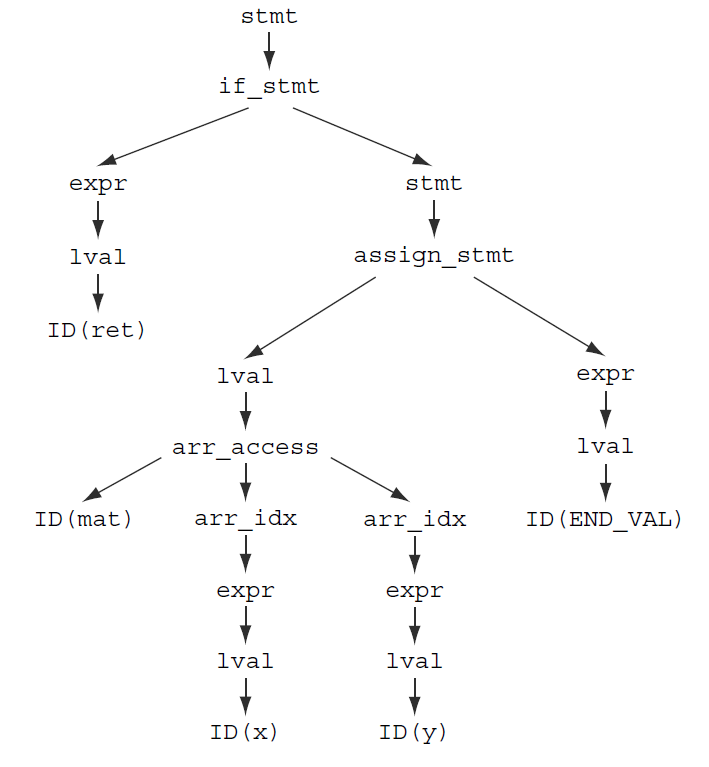
\includegraphics[width=0.8\textwidth]{Imagens/Arvore}
		\label{fig:TreeParser}
		\caption{Árvore de parser.}
	\end{figure}
	
	
	\subsection{Paser JDT Eclipse}
	No caso do \textit{parser} provido pela infraestrutura \textit{JDT} do eclipse,  a classe \textit{ASTParser} contida na biblioteca \textit{org.eclipse.jdt.core.dom} permite a criação de uma árvore de sintaxe abstrata.\\
	Este procedimento é realizado em todos os aquivos \textit{.java} contido em um projeto e com isso cada um possui uma referência de \textit{CompilationUnit} o qual permite acesso ao nó raiz árvore sintática de cada arquivo. O parse é gerado conforme as últimas definições da linguagem utilizando \textit{AST.JLS8}.\

	\begin{lstlisting}
		ASTParser parser = ASTParser.newParser(AST.JLS8);
		
		Map<String, String> options = JavaCore.getOptions();
		options.put(JavaCore.COMPILER_COMPLIANCE, JavaCore.VERSION_1_8);
		options.put(JavaCore.COMPILER_CODEGEN_TARGET_PLATFORM, JavaCore.VERSION_1_8);
		options.put(JavaCore.COMPILER_SOURCE, JavaCore.VERSION_1_8);
		
		parser.setKind(ASTParser.K_COMPILATION_UNIT);
		parser.setCompilerOptions(options);
		parser.setSource(contents);
		
		final CompilationUnit cu = (CompilationUnit) parser.createAST(null);
		return cu;
	\end{lstlisting}
	
	Neste, o \textit{parser} é realizado através de uma classe denominada de mesmo nome, a qual é instanciada um única vez no projeto através do padrão \textit{singleton} \cite{Gamma:1995}.
	

	\section{Sintaxe abstrata}
	É possível fazer uma análise significativa em uma árvore de parser, e certos tipos de checagem estilísticas são mais bem executadas em uma árvore de análise, pois contém mais representações diretas do código assim como o programador escreve. No entanto, executar análise complexa em uma árvore de análise pode ser inconveniente. Os nós da árvore são derivados diretamente das regras de produção da gramática, e essas regras podem-se introduzir símbolos não terminais que existem apenas para fins de fazer a análise mais fácil e menos ambígua, ao invés de para o objetivo de produzir uma facilmente compreendido a árvore. É geralmente melhor para abstrair ambos os detalhes da gramática e as estruturas sintáticas presente no código fonte do programa. Uma estrutura de dados que faz estas coisas é chamado de uma árvore de sintaxe abstrata (AST). O objectivo da AST é fornecer uma versão padronizada do programa adequado para posteriores análises. A AST é normalmente construída associando código construção árvore com regras de produção da gramática. A Figura: \ref{fig:ArvoreAST} mostra uma AST. Observa-se que a instrução {\it if} agora tem uma outra ramificação vazia, o predicado testado pelo caso é agora uma comparação explícita para zero (o comportamento exigido pelo C), e acesso à matriz é uniformemente representada como uma operação de binário.
	
	\begin{figure}[h]
		\center
		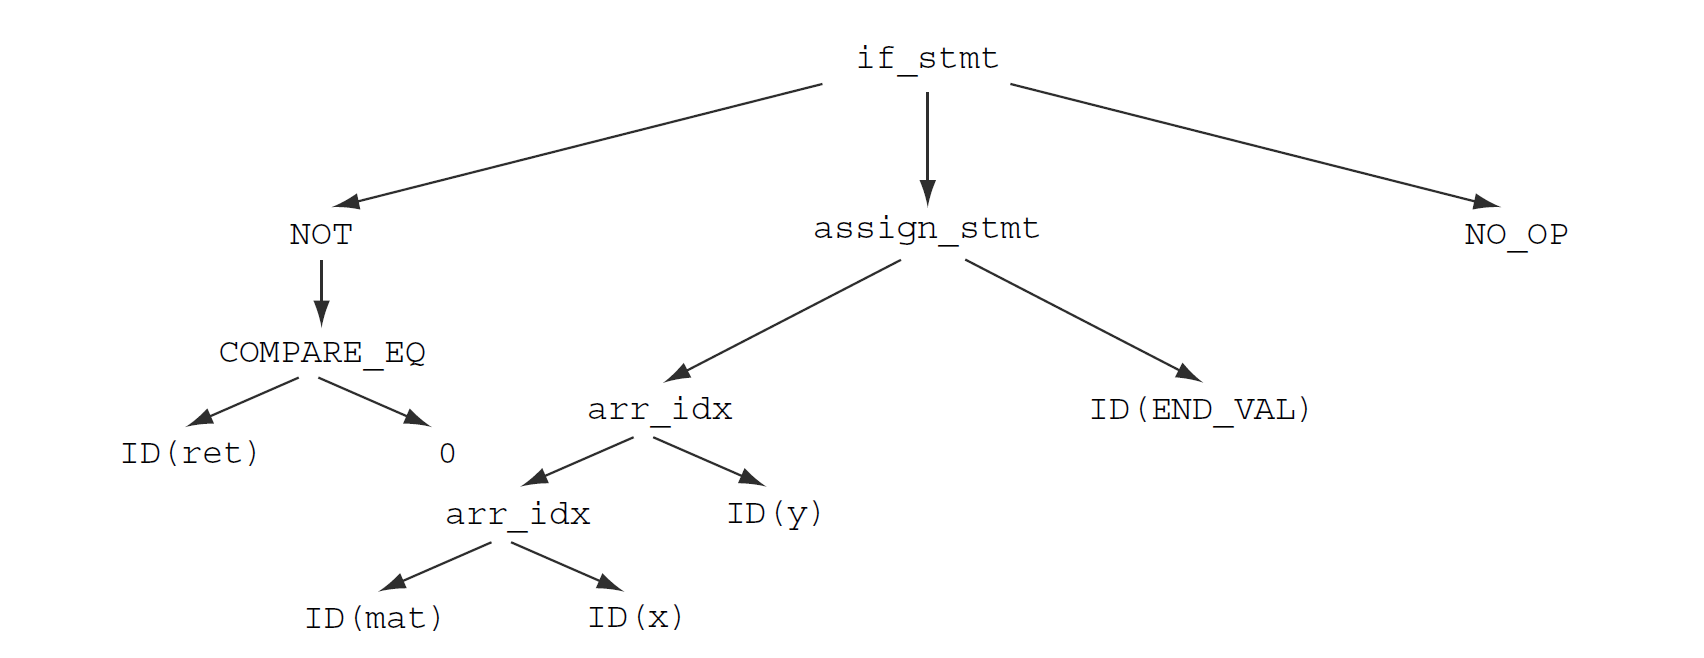
\includegraphics[width=1\textwidth]{Imagens/ArvoreAST}
		\label{fig:ArvoreAST}
		\caption{Árvore AST.}
	\end{figure}

	\section{Análise semântica}
	Como a AST está sendo construída, a ferramenta cria uma tabela de símbolos ao lado dela. Para cada identificador no programa, a tabela de símbolos associa o identificador com seu devido tipo e um ponteiro para a sua declaração ou definição. Com a AST e a tabela de símbolo, a ferramenta está agora equipado-se para realizar a verificação de tipo. A ferramenta de análise estática não pode ser obrigados a comunicar erros de checagem de tipo da maneira um compilador faz, mas informações de tipo é criticamente importante para a análise de uma linguagem orientada a objetos, porque o tipo de um objeto determina o conjunto de métodos que o objeto pode invocar. Além disso, é normalmente desejável para converter, pelo menos, as conversões do tipo implícito no código fonte para conversões de tipo explícitas no AST. Por estas razões, uma ferramenta de análise estática avançado tem a ver apenas como muito trabalho relacionado com a verificação de tipo como um compilador faz. No mundo do compilador, resolução de símbolo e verificação de tipo são referidos como análise semântica porque o compilador está atribuindo significado aos símbolos encontrada no programa. As ferramentas de análise estática que usam essas estruturas de dados têm uma vantagem distinta sobre ferramentas que não o fazem. Por exemplo, eles podem interpretar corretamente o significado dos operadores sobrecarregados em C++ ou determinar que um método em Java chamado doPost () é, na verdade, uma parte de uma implementação de HttpServlet.Estas capacidades permitem uma ferramenta para executar verificações úteis na estrutura deo programa. Após análise semântica, compiladores e a análise estática mais avançada ferramentas de formas de peça. Um compilador moderno usa a AST e o símbolo e o tipo informações para gerar uma representação intermediaria, uma versão genérico do código de máquina que é adequado para otimização e, em seguida, a conversão em específico da plataforma de código-objeto. O caminho para ferramentas de análise estática é menos clara. Dependendo do tipo de análise a ser realizada, uma ferramenta de análise estática pode executar transformações adicionais sobre a AST ou pode gerar a sua própria variedade de representação intermediária adequada às suas necessidades. Se uma ferramenta de análise estática usa sua própria representação intermediária, que, geralmente, permite a atribuição, pelo menos, ramificando, {\it looping}, e chamadas de função. A representação intermediária que uma ferramenta de análise estática usa é geralmente umvista de nível superior do programa do que a representação intermediária que um compilador usa. Por exemplo, um compilador de linguagem C, provavelmente, converter todas as referências a campos para estruturar deslocamentos em {\it byte} na estrutura pela sua representação intermediaria, enquanto uma ferramenta de análise estática mais provavelmente continuará para se referir a estrutura de campos, pelos seus nomes.